\documentclass[12pt,a4paper]{article}

\usepackage[utf8]{inputenc}
\usepackage[T1]{fontenc}
\usepackage{lmodern}
\usepackage[margin=1in]{geometry}
\usepackage{setspace}
\usepackage{graphicx}
\usepackage{hyperref}
\usepackage{booktabs}
\usepackage{amsmath}
\usepackage{subcaption}
\usepackage{caption}
\usepackage{microtype}
\captionsetup{font=small, labelfont=bf}
\captionsetup[subfigure]{font=small}

\onehalfspacing

\hypersetup{colorlinks=true, linkcolor=blue, citecolor=blue, urlcolor=blue}

\title{\textbf{Communication Tone in Pull Request Discussions:\\
Associations with Merge Outcomes and Contributor Return}}
\author{Dimitrios Stamatios Bouras \\
        Student ID: 2501112125 \\[2pt]
        \small Quantitative Analysis of Open Source Software, Spring 2026 \\
        \small Peking University}
\date{}

\begin{document}
\maketitle
\thispagestyle{empty}

\begin{abstract}
\noindent
Does the tone of a code review discussion shape whether a pull request gets merged, and whether the contributor comes back? This study takes an empirical approach to a widely held belief in open source communities: that hostile or discouraging reviews drive contributors away. Using a dataset of 12,098 focal pull requests (PRs) from three major repositories --- Kubernetes, Next.js, and scikit-learn --- we score over 100,000 review comments with transformer-based NLP models for toxicity, sentiment, and anger, and with a lexical heuristic for politeness, then fit logistic regression models with structural and contributor-history controls. The central finding is a sharp asymmetry: communication tone strongly associates with \emph{whether a PR is accepted}, but plays almost no role in \emph{whether the author returns}. Positive sentiment is the dominant predictor of merge ($\beta = 2.10$, $p < 10^{-60}$), while return at 90 days is overwhelmingly explained by prior contribution history ($\beta = 1.51$, $p < 10^{-179}$). Overt toxicity affects only 1\% of PRs and does not produce a stable association with return. A significant politeness moderation effect ($p = 0.003$) suggests that overall community tone buffers the impact of isolated harsh moments. These findings reframe the retention problem: in well-moderated communities, the primary risk is insufficient early onboarding, not individual harsh reviews.
\end{abstract}

\hrule
\vspace{0.5em}

% ── 1. Introduction ─────────────────────────────────────────────
\section{Introduction}

A common narrative in open source software (OSS) communities holds that toxic or discouraging review feedback drives contributors away, and that this effect is especially severe for newcomers. Codes of conduct, welcoming committees, and reviewer guidelines are all policy responses to this belief. Yet the empirical evidence is thin: most studies of OSS contributor retention are qualitative, focus on self-reported barriers, or measure broad social dynamics rather than specific measurable signals in individual PR discussions~\cite{steinmacher2015, tourani2017}.

This project asks a more precise version of the question: do \emph{measurable} communication signals --- toxicity, sentiment, anger, politeness --- in pull request review discussions associate with (a) whether the PR gets merged and (b) whether the author opens another PR within a follow-up window? And if they do, do these associations differ for newcomers versus experienced contributors?

We frame four research questions. \textbf{RQ1:} Which communication signals associate with PR merge outcome? \textbf{RQ2:} Which signals associate with author return at 30, 90, and 180 days? \textbf{RQ3:} Are newcomers more sensitive to harsh language than experienced contributors? \textbf{RQ4:} Does overall discussion politeness moderate the association between toxicity and return?

The study is explicitly observational. We estimate associations in naturally occurring data under structural controls, not causal effects from randomized experiments. This framing is not a weakness but a design choice: the goal is to establish what is actually associated with outcomes in large, active repositories before any intervention claim is made.

% ── 2. Data Collection ─────────────────────────────────────────
\section{Data Collection}

\subsection{Repository selection and collection window}

Three repositories were chosen to balance diversity and scale: \texttt{kubernetes/kubernetes} (infrastructure, large and busy), \texttt{vercel/next.js} (web framework, commercially backed), and \texttt{scikit-learn/scikit-learn} (scientific Python, community governed). All three are well-moderated, high-traffic projects where PR review is a formal process --- making them good candidates for studying communication effects.

Pull request metadata and comment text were collected via the GitHub REST API across a total window of July 2023 to September 2025. The window is divided into three sub-periods that serve distinct purposes:

\begin{itemize}\setlength\itemsep{2pt}
  \item \textbf{Lookback (Jul--Dec 2023):} Used exclusively to compute contributor history before any focal PR is observed. Without this buffer, a contributor who opened their first PR in January 2024 would be classified as a newcomer correctly; but without the lookback, someone who had been contributing since October 2023 might be misclassified. The lookback prevents this data leakage in newcomer classification.
  \item \textbf{Focal window (Jan 2024--Mar 2025):} The 12,098 PRs that enter the analysis --- the events we are trying to predict.
  \item \textbf{Follow-up (Mar--Sep 2025):} Provides complete 90-day and 180-day return labels for the latest focal PRs; without it, recent PRs would be right-censored.
\end{itemize}

The final dataset covers 12,098 focal PRs by 2,210 distinct authors, with over 100,000 scored reviewer comments. Table~\ref{tab:desc} reports repository-level statistics.

\begin{table}[h]
\centering
\caption{Repository-level descriptive statistics.}
\label{tab:desc}
\small
\begin{tabular}{lrrrr}
\toprule
\textbf{Repository} & \textbf{$N$ PRs} & \textbf{Merge \%} & \textbf{Toxic$\geq$0.05 (\%)} & \textbf{Newcomer \%} \\
\midrule
kubernetes/kubernetes     & 4{,}713 & 70.7 & 2.0 & 17.1 \\
vercel/next.js            & 6{,}248 & 79.7 & 0.3 & 15.4 \\
scikit-learn/scikit-learn & 1{,}137 & 74.1 & 0.6 & 27.2 \\
\midrule
\textbf{All repos}        & 12{,}098 & 75.7 & 1.0 & 17.2 \\
\bottomrule
\end{tabular}
\end{table}

A descriptive finding that shapes all subsequent modelling: overt toxicity is extremely rare. Only 1.0\% of PRs contain any reviewer comment with a toxicity score at or above 0.05. The overall 90-day return rate is 81.3\%; the prior PR count has mean 65.7 and SD 96.1 --- a very wide spread that motivates log-transformation in regressions.

\subsection{Preprocessing and comment filtering}

Before NLP scoring, each comment is preprocessed: code blocks, inline code, URLs, and \texttt{@mentions} are stripped. Only \emph{received} comments are retained --- comments written by reviewers other than the PR author, after bot accounts are removed by login pattern. This ensures that the NLP signals capture the tone of the feedback the PR author received, not their own writing style.

% ── 3. Research Pipeline ────────────────────────────────────────
\section{Research Pipeline}

\subsection{NLP signal extraction}

Four communication signals are computed per comment and then aggregated to the PR level:

\begin{itemize}\setlength\itemsep{2pt}
  \item \textbf{Toxicity:} scored with \texttt{unitary/toxic-bert}~\cite{hanu2020}. Aggregated as both the maximum toxicity score across all reviewer comments (\texttt{max\_toxicity\_x100}, scaled by 100 for coefficient readability) and binary flags at thresholds 0.05 and 0.10.
  \item \textbf{Sentiment:} scored with \texttt{cardiffnlp/twitter-roberta-base-sentiment-latest}~\cite{barbieri2020}, expressed as $P(\text{positive}) - P(\text{negative}) \in [-1, 1]$, averaged across comments.
  \item \textbf{Anger:} scored with \texttt{j-hartmann/emotion-english-distilroberta-base}~\cite{hartmann2022}, a six-emotion classifier. The anger probability is averaged across comments.
  \item \textbf{Politeness:} computed as a lexical marker density --- a count of explicit courtesy markers (``please'', ``thank you'', ``could you'', ``would you mind'', etc.) normalised by $\log(1 + \text{word count})$. This is a simple heuristic, not a model; it captures surface-level hedging and courtesy language.
\end{itemize}

The maximum rather than mean is used for toxicity because the distribution is severely right-skewed (mean $\approx 0.001$, max $\approx 0.003$ even at the 99th percentile). Averaging near-zero scores loses almost all signal; the worst-comment score is the operationalisation most likely to reflect a contributor's experience of the discussion.

\subsection{Regression model and controls}

Both primary outcomes are binary: \texttt{merged} (0/1) and \texttt{returned\_N} (0/1 for $N \in \{30, 90, 180\}$ days). Logistic regression is used throughout, with HC3 heteroskedasticity-robust standard errors. Variance inflation factors range from 1.01 to 1.25, confirming no meaningful multicollinearity among the communication variables.

All models include the following controls:
\begin{itemize}\setlength\itemsep{2pt}
  \item \textbf{Contributor history:} $\log(\text{prior PR count})$ and a binary \texttt{is\_newcomer} indicator (no PRs in the lookback window)
  \item \textbf{Discussion structure:} $\log(\text{number of received comments})$, number of distinct participants, $\log(\text{first response delay in hours})$
  \item \textbf{Repository fixed effects}
\end{itemize}

For RQ3 and RQ4, interaction terms are added to the 90-day return model: \texttt{max\_toxicity $\times$ is\_newcomer} and \texttt{max\_toxicity $\times$ mean\_politeness} respectively.

% ── 4. Results ──────────────────────────────────────────────────
\section{Results}

\subsection{RQ1: What predicts merge?}

The merge model ($N = 12{,}098$, McFadden pseudo-$R^2 = 0.118$) yields three significant communication findings (Table~\ref{tab:merge}).

\begin{table}[h]
\centering
\caption{Selected logistic regression coefficients for PR merge outcome.}
\label{tab:merge}
\small
\begin{tabular}{lrrr}
\toprule
\textbf{Variable} & \textbf{Coef.} & \textbf{95\% CI} & \textbf{$p$} \\
\midrule
mean\_sentiment           & $+2.10$ & [1.87,\; 2.34]         & $<10^{-60}$ \\
mean\_anger               & $+4.40$ & [3.47,\; 5.32]         & $<10^{-20}$ \\
mean\_politeness          & $-1.42$ & [$-1.82$,\; $-1.03$]   & $<10^{-12}$ \\
max\_toxicity\_x100       & $+0.031$& [0.004,\; 0.058]       & 0.026       \\
log\_prior\_pr\_count     & $+0.296$& [0.258,\; 0.334]       & $<10^{-52}$ \\
\bottomrule
\end{tabular}
\end{table}

Positive sentiment is the strongest communication predictor of merge, as one might expect. More surprising are the directions of anger and politeness. \textbf{Anger is positively associated with merge} because the emotion model was trained on social media: assertive technical language such as ``this is completely broken'' or ``this implementation is wrong'' scores high on anger in that domain, but in code review it signals \emph{engaged, decisive review} that pushes a PR toward a decision. \textbf{Politeness is negatively associated with merge} because hedged language --- ``maybe consider\ldots'', ``not sure if this is the right approach\ldots'', ``could you perhaps\ldots'' --- is the register reviewers use to soften rejection. It marks discomfort with the code, not approval of it.

This is the central methodological lesson of the project: NLP signals carry real information about PR discussions, but not necessarily the information they were designed to capture. Domain context is essential for interpretation. The same lexical and acoustic features mean different things in code review than in social media discourse.

\subsection{RQ2: What predicts contributor return?}

The return model tells a strikingly different story (Table~\ref{tab:return}). Prior PR count is the dominant predictor by an enormous margin, with pseudo-$R^2 = 0.498$ at 90 days driven almost entirely by that single variable.

\begin{table}[h]
\centering
\caption{Selected logistic regression coefficients for 90-day contributor return.}
\label{tab:return}
\small
\begin{tabular}{lrrr}
\toprule
\textbf{Variable} & \textbf{Coef.} & \textbf{95\% CI} & \textbf{$p$} \\
\midrule
log\_prior\_pr\_count & $+1.51$ & [1.41,\; 1.61]       & $<10^{-179}$ \\
mean\_anger           & $+5.54$ & [3.86,\; 7.22]       & $<10^{-10}$  \\
mean\_sentiment       & $+0.020$& [$-0.27$,\; 0.31]    & 0.89         \\
mean\_politeness      & $-0.385$& [$-0.93$,\; 0.16]    & 0.17         \\
max\_toxicity\_x100   & $+0.034$& [$-0.024$,\; 0.093]  & 0.25         \\
\bottomrule
\end{tabular}
\end{table}

Toxicity, sentiment, and politeness are all non-significant. The model that explains half the variance in 90-day return does so without them. Whether a contributor comes back is overwhelmingly a function of \emph{who they already were} before the focal PR --- their level of embeddedness in the project --- not of what happened in any given review discussion.

\begin{figure}[h]
\centering
\begin{subfigure}[t]{0.47\textwidth}
  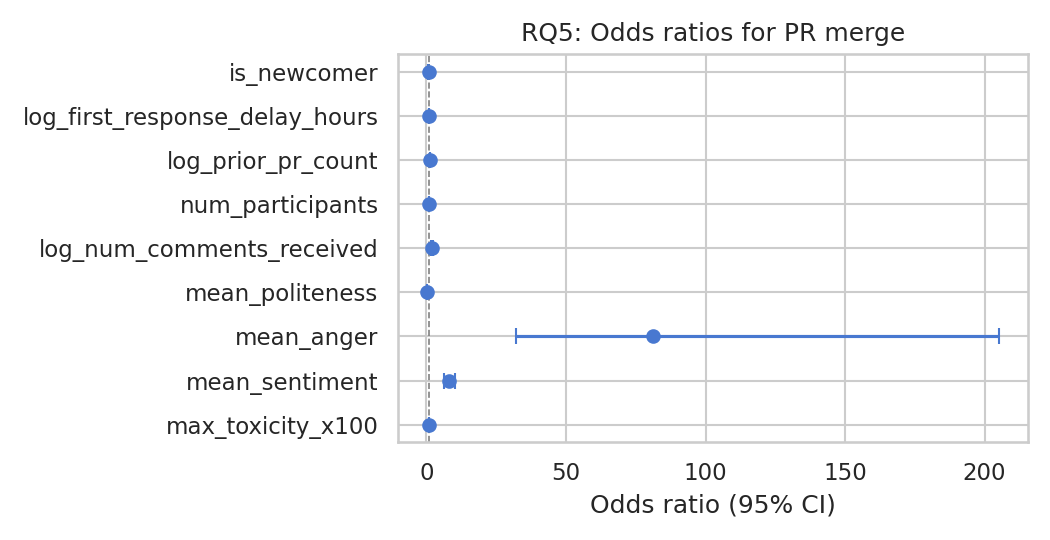
\includegraphics[width=\linewidth]{results/figures/06a_coef_merge.png}
  \caption{Merge outcome (pseudo-$R^2 = 0.118$)}
\end{subfigure}
\hfill
\begin{subfigure}[t]{0.47\textwidth}
  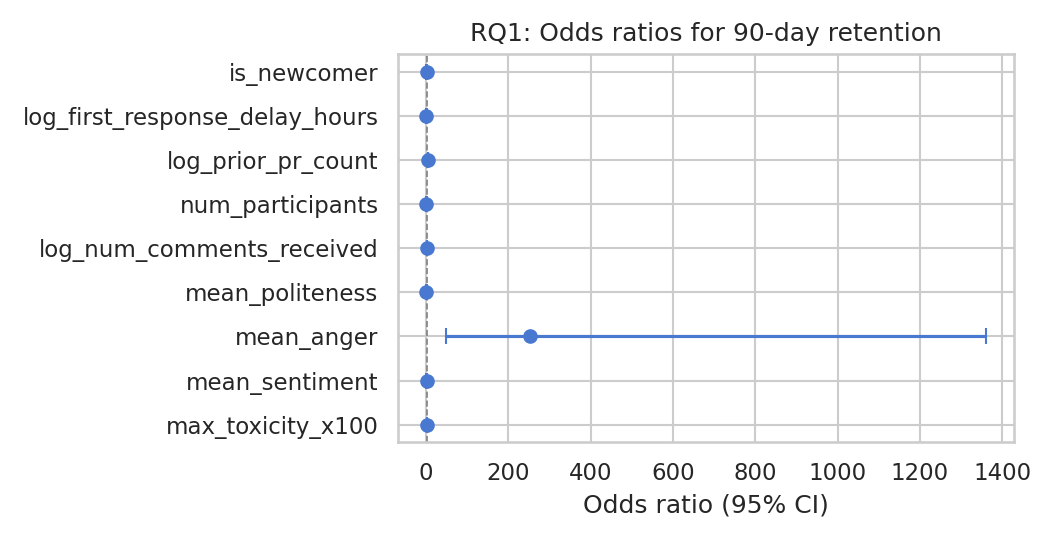
\includegraphics[width=\linewidth]{results/figures/06b_coef_retention90.png}
  \caption{90-day return (pseudo-$R^2 = 0.498$)}
\end{subfigure}
\caption{Logistic regression coefficients with 95\% confidence intervals. In the merge model (left), sentiment and anger dominate and politeness is the largest negative predictor. In the return model (right), prior PR count dwarfs all communication signals, which cluster near zero with wide confidence intervals.}
\label{fig:coefs}
\end{figure}

\subsection{RQ3: Are newcomers more sensitive to harsh language?}

To test differential sensitivity, we add a \texttt{max\_toxicity $\times$ is\_newcomer} interaction to the 90-day return model. The interaction is not significant ($\beta = 0.029$, $p = 0.57$). Newcomers return at far lower rates ($\sim$28\%) than experienced contributors ($\sim$92\%), but this gap is explained entirely by their shorter prior history, not by differential sensitivity to the tone they received.

Notably, as Figure~\ref{fig:newcomer} shows, toxicity \emph{exposure} is similar for both groups: newcomers are not treated more harshly. The massive return-rate gap ($28\%$ vs.\ $92\%$) is therefore not a communication problem --- it is an embeddedness problem. Contributors who have made many prior contributions return almost regardless of how a single PR discussion went; newcomers who have made none are at risk of not returning even after entirely civil discussions.

\begin{figure}[h]
\centering
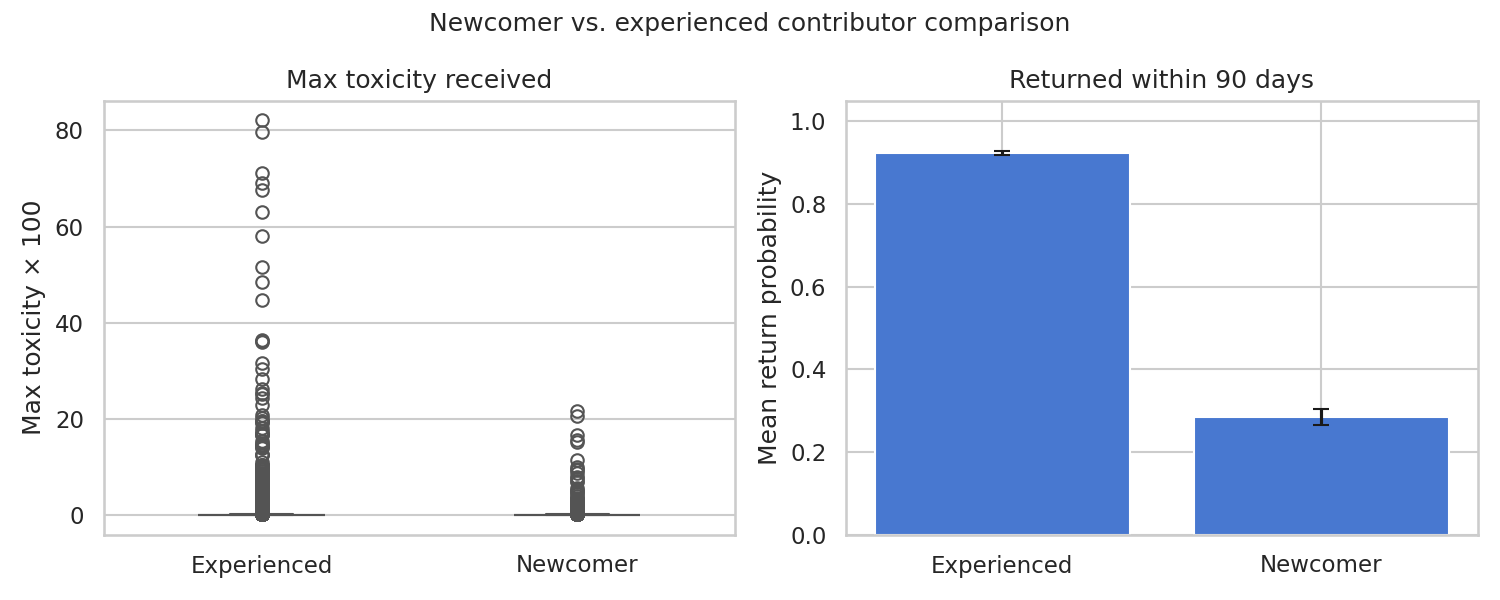
\includegraphics[width=0.80\textwidth]{results/figures/05_newcomer_vs_experienced.png}
\caption{Newcomer vs.\ experienced contributor comparison. Left: the distribution of max toxicity received is similar for both groups. Right: 90-day return rate is $\sim$92\% for experienced contributors and $\sim$28\% for newcomers. The interaction between toxicity and newcomer status is not significant ($p = 0.57$), confirming that the gap is about contribution history, not communication tone.}
\label{fig:newcomer}
\end{figure}

\subsection{RQ4: Does politeness buffer isolated harsh language?}

Adding a \texttt{max\_toxicity $\times$ mean\_politeness} interaction to the 90-day return model yields a significant positive coefficient ($\beta = 0.81$, $p = 0.003$). When the surrounding discussion is polite overall, isolated harsh comments are less negatively associated with return. The overall culture of the thread appears to absorb individual difficult moments.

This is the one result that fits the intuitive community-health narrative, but it operates at the level of the \emph{discussion context} rather than any individual comment. A single sharp remark in an otherwise civil conversation is less damaging than the same remark in a hostile thread.

\subsection{Robustness checks}

Replacing continuous max toxicity with binary flags produces threshold-sensitive results: the 0.05 indicator is significant in the return model ($\beta = 1.38$, $p < 0.001$), while the 0.10 indicator is not ($p = 0.15$). This confirms that toxicity effects are both sparse and operationalization-sensitive. The data do not support a stable ``toxic comments drive contributors away'' narrative --- the conclusion depends heavily on where the threshold is drawn.

% ── 5. Experience ───────────────────────────────────────────────
\section{Experience}

The most valuable lesson was about the limits of ready-made NLP tools. I began expecting emotion and politeness scores to be interpretable at face value --- angry comments would hurt merge, polite comments would help. Both signals turned out to carry \emph{inverted} associations with merge outcomes. Tracing the cause --- domain shift from social media training data to code review discourse --- was the intellectual turning point of the project, and it forced a much more careful reading of what these models actually measure.

The hardest technical challenge was toxicity sparsity. When 99\% of the data is at or near zero, operationalisation choices matter enormously: switching from mean to maximum toxicity, and from continuous to binary flags at different thresholds, changed significance. A second non-trivial design decision was the lookback period: without a six-month buffer of pre-focal history, contributors who had started shortly before the analysis window would be misclassified as newcomers, leaking future information into a key control variable.

If I were starting again, I would invest in a small manual annotation of 200--300 comments for code-review-relevant tone before committing to off-the-shelf NLP models. Having domain-specific ground truth would let me validate the signals rather than discovering their quirks through counterintuitive regression signs.

% ── 6. Traces During the Project ────────────────────────────────
\section{Traces During the Project}

The full project --- data collection scripts, NLP scoring pipeline, analysis code, and this report --- is archived in a GitHub repository:

\begin{center}
\url{https://github.com/jimbou/oss-analysis-2501112125}
\end{center}

The repository contains: (1) five Python scripts covering the full pipeline from GitHub API collection to logistic regression output; (2) all NLP-scored comment data and PR-level aggregations; (3) regression result tables and coefficient figures; (4) this report; and (5) documentation files describing the data schema, pipeline steps, and how to interpret the results. All HuggingFace model identifiers are pinned; setup instructions are in \texttt{README.md}.

% ── 7. Conclusion ───────────────────────────────────────────────
\section{Conclusion}

Communication tone is more strongly associated with \emph{merge outcomes} than with \emph{contributor return}. Positive sentiment dominates the merge model; prior contribution history dominates the return model to a degree that leaves toxicity, sentiment, and politeness all non-significant. Newcomers and experienced contributors face similar toxicity levels, but newcomers return at 28\% versus 92\% for experienced contributors --- a gap driven by embeddedness, not communication. The one community-health finding that holds is the politeness moderation: an overall polite thread buffers the impact of isolated harsh comments.

The practical upshot is that improving retention requires investing in early onboarding, not policing individual review conversations. A contributor with deep history is resilient to a single harsh review; a newcomer with none is at risk regardless of tone. The methodological upshot is that off-the-shelf NLP models carry domain-specific biases that can invert expected associations in code review; domain validation is not optional.

% ── References ──────────────────────────────────────────────────
\section*{References}

\begingroup
\small
\setlength{\parskip}{3pt}

\noindent [1] \label{hartmann2022} Hartmann, J. (2022). \textit{Emotion English DistilRoBERTa-base}. HuggingFace. \url{https://huggingface.co/j-hartmann/emotion-english-distilroberta-base}

\noindent [2] \label{hanu2020} Hanu, L., \& Unitary Team (2020). \textit{Detoxify}. GitHub. \url{https://github.com/unitaryai/detoxify}

\noindent [3] \label{barbieri2020} Barbieri, F., Camacho-Collados, J., Espinosa-Anke, L., \& Neves, L. (2020). TweetEval: Unified benchmark and comparative evaluation for tweet classification. \textit{Findings of EMNLP}, 1644--1650.

\noindent [4] \label{steinmacher2015} Steinmacher, I., Silva, M.\,A.\,G., Gerosa, M.\,A., \& Redmiles, D.\,F. (2015). A systematic literature review on the barriers faced by newcomers to open source software projects. \textit{Information and Software Technology}, 59, 67--85.

\noindent [5] \label{tourani2017} Tourani, P., Adams, B., \& Serebrenik, A. (2017). Code of conduct in open source projects. \textit{Proceedings of SANER}, 24--33.

\endgroup

\end{document}
